\documentclass[aspectratio=169]{beamer}
\usetheme{Madrid}
\usepackage[utf8]{inputenc}
\usepackage[T1]{fontenc}
\usepackage{tikz}
\usepackage{amssymb}
\usepackage{graphicx}
\setbeamertemplate{navigation symbols}{}
\setbeamercolor{title}{fg=white,bg=magenta!70!red}
\setbeamercolor{frametitle}{fg=white,bg=magenta!70!red}
\setbeamercolor{block title}{bg=magenta!70!red!20,fg=black}
\setbeamercolor{block body}{bg=magenta!70!red!8,fg=black}
\setbeamercolor{item}{fg=magenta!70!red}
\setbeamercolor{itemize item}{fg=magenta!70!red}
\setbeamertemplate{itemize item}[triangle]

\title{Foundations 2 — Binary (Unplugged)}
\subtitle{What is binary? Transistors, addition, and the classic binary cards}
\author{ByteForge --- Grade 9 --- The Deep Diver}
\date{}

\begin{document}

\begin{frame}
    \titlepage
\end{frame}

\begin{frame}{Today's Missions}
    \Large
    \begin{itemize}
        \item Learn: What Is Binary?
        \item Binary Cards --- Make the Number
        \item Binary Cards --- Addition
        \item BOSS: Bigger Numbers
    \end{itemize}
\end{frame}

\begin{frame}{A transistor is a tiny ON/OFF switch}
    \large
    \begin{itemize}
        \item Billions of these inside every chip --- each one is either ON or OFF, nothing in between
        \item ON = 1, OFF = 0 --- that is the ENTIRE alphabet a computer actually uses
        \item "Binary" just means "made of only two symbols"
    \end{itemize}
\end{frame}


\begin{frame}{Each binary place is worth double the last}
    \large
    \begin{itemize}
        \item 1, 2, 4, 8, 16, 32, 64, 128 --- powers of 2, doubling every step left
        \item A binary digit only counts if it is a 1 --- flip a card face-up to "add" its value
        \item 22 = 16 + 4 + 2 --- so 22 in binary is 10110
    \end{itemize}
\end{frame}


\begin{frame}{Binary addition works with real carrying}
    \large
    \begin{itemize}
        \item 1 + 1 in one place = 0, carry 1 to the next place --- same idea as carrying in denary addition
        \item The card trick makes this physical: flip cards until their total matches the target number
    \end{itemize}
\end{frame}

\begin{frame}{Real-World Examples}
    \large
    \begin{itemize}
        \item Every single photo, song, and message on your phone is stored as nothing but 1s and 0s underneath --- this unplugged activity IS the real mechanism, just done by hand.
        \item A dimmer light switch is NOT binary (it has many in-between levels) --- but a normal light switch genuinely is: only ON or OFF, exactly like one bit.
    \end{itemize}
\end{frame}


\begin{frame}{Image}
    \begin{center}
    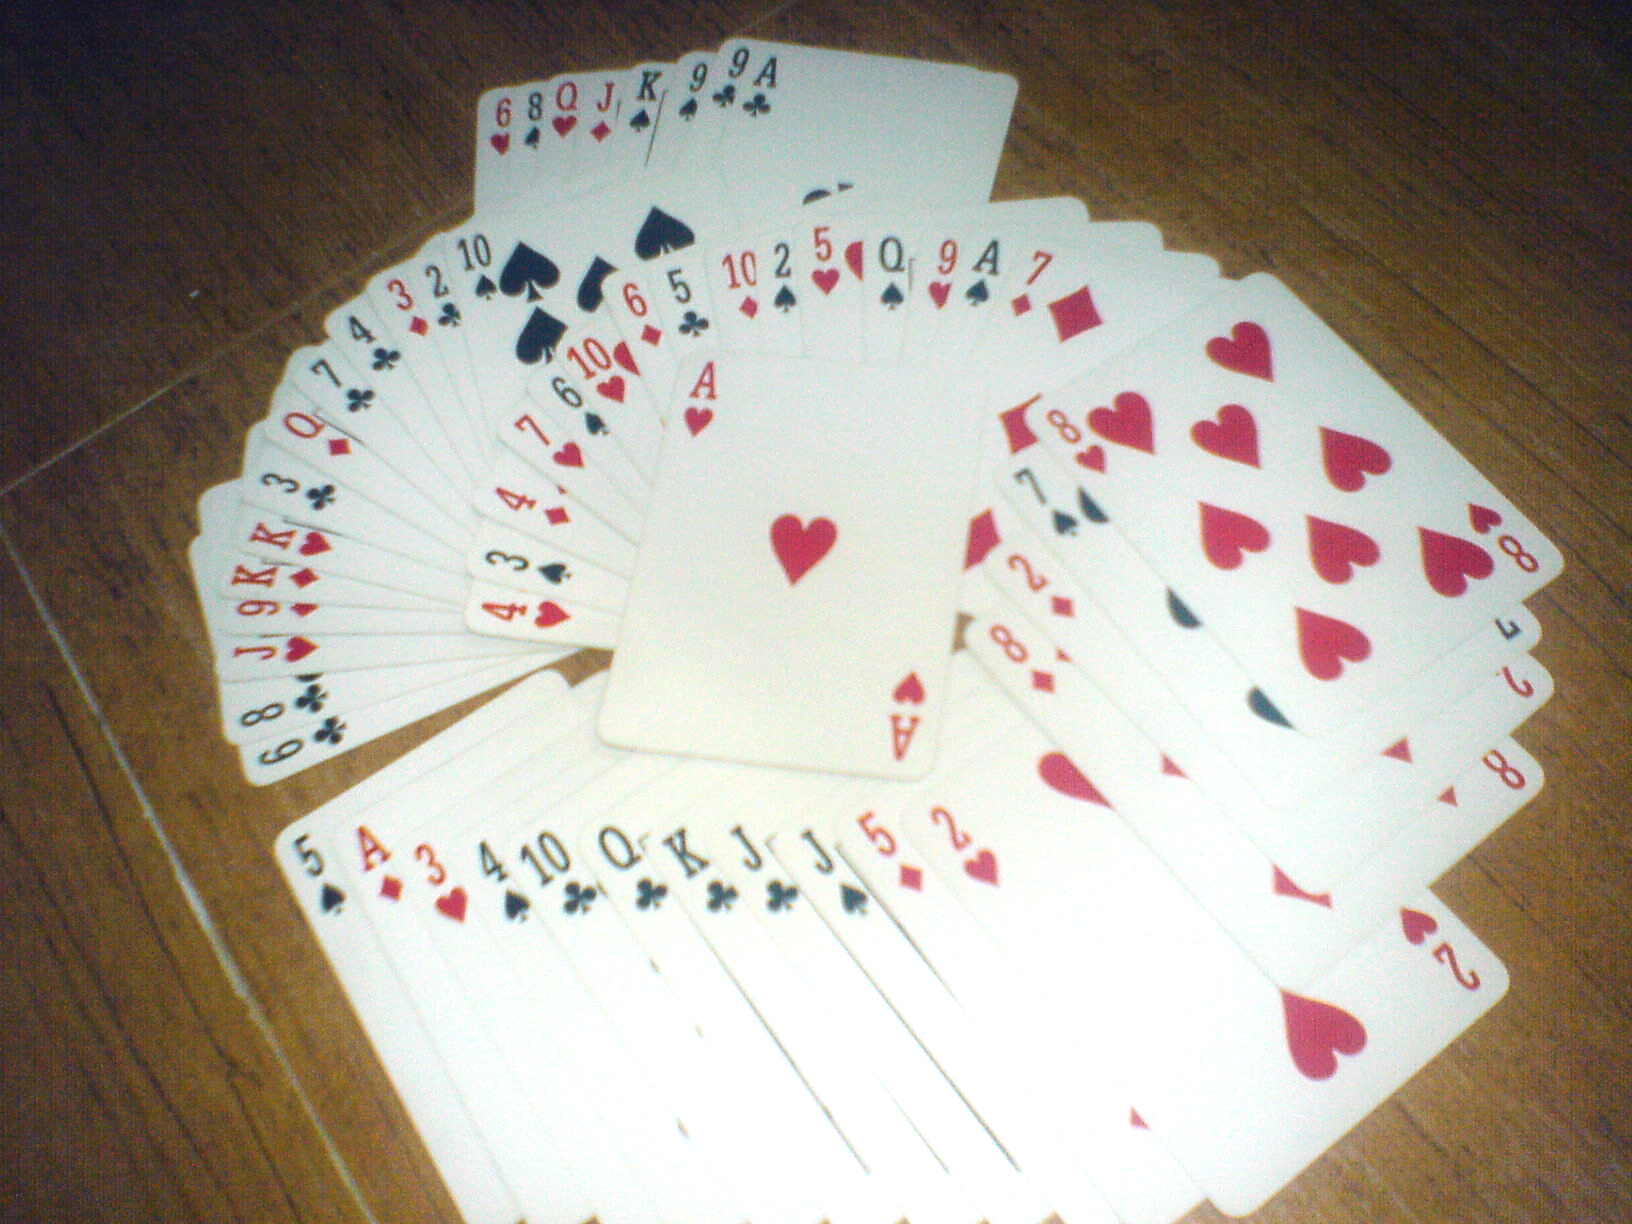
\includegraphics[width=0.5\textwidth]{images/cards.jpg}

    \large Real playing cards fanned out --- the same "flip to include, hide to exclude" idea as the binary cards activity.

    \small Playing cards --- Imager Visioner, public domain, via Wikimedia Commons
    \end{center}
\end{frame}

\begin{frame}{Let Them Discover (1/2)}
    \large
    Before touching the platform: as a class, physically flip real cards (or paper squares) labelled 16, 8, 4, 2, 1 to build the number 22. Which cards ended up face-up?
\end{frame}


\begin{frame}{Let Them Discover (2/2)}
    \large
    Find a real switch in the room that is genuinely binary (only 2 states) and one that is NOT (has a range). What tells them apart?
\end{frame}

\begin{frame}{Your Turn}
    \Large
    Open the mission map, find \textbf{Foundations 2 — Binary (Unplugged)}, and fly it for real ---
    everything you just saw, you now do yourself.
\end{frame}

\end{document}
